
\section{Geographic Information System | Nurul Izza Hamka | 1174062}
\subsection{Buku}
Buku Belum Lunas
\subsection{Pengertian Sistem Informasi geografis}
\begin{enumerate}

\item Pemahaman Pada Sistem Informasi Geografis

Sistem Informasi Geografis merupakan pemahaman dari 3 rangkaian kata, sebagai berikut:\\
1. Geogarfi\\
Sistem Informasi Geografis dibangun berdasarkan pada istilah 'geografi' atau 'spasial'. Objek mengacu pada sfesifikasi  lokasi dalam suatu ruang/tempat. Objek dapat berupa fisik, budaya ataupun ekonomi alamiah.\\
2. Informasi\\
Informasi berasal dari kata pengelohan sejumlah data. Didalam sistem informasi geografis informasi mempunyai volume terbesar. Dan setiap object geografi memiliki setting datanya tersendiri karena tidak sepenuhnya data yang ada dapat terwakili di dalam peta. Maka, semua data harus diasosiasikan pada objek spasial yang mampu membuat peta menjadi intelligent.\\
3.Sistem\\
pengertian dari suatu sistem merupakan kumpulan elemen-elemen yang saling berintegrasi dan berinterdependensi dalam sebuah lingkungan yang dinamis untuk mencapai tujuan tertentu.\\

\item Definisi Sistem Informasi Geografis (Geographic Information System) 

Sistem informasi geografis adalah sebuah komputer yang berbasis sistem informasi yang digunakan untuk memberikan informasi bentuk digital dan analisa terhadap permukaan geografi bumi. \\
Sistem informasi geografis (GIS) diartikan sebagai sistem untuk penyimpanan, memerikas, mengintegrasi, memanipualasi, menganalisis dan memaparkan data yang berkaitan denagn semua ruang yang berhubungan dengan keadaan bumi.\\
Geografis adalah bidang kajian ilmu dan teknologi yang masih abru. Ada beberapa definisi dari Sistem Informasi Geograpis yaitu :\\
a. Definisi SIG menurut (Rhind, 1998) yaitu GIS is a computer system for collecting, integrating and analyzing information related to the surface of the earth.\\
b. Definisi SIG menurut (Marble dan Peuquet, 1983) and (Parker, 1988; Ozemoy et al.,1981; Burrough,1986) yaitu GIS deals with space-time data and often but notnecessarily, employs computer hardware and software)\\

\end{enumerate}
\subsection{Sejarah}
\begin{enumerate}
\item Peta\\
Peta merupakan penggambaran secara grafis atau bentuk skala (perbandingan) pada konsep mengenai bumi dalam hal ini peta merupakan alat untuk menyampaikan atau menginformasikan mengenai ilmu kebumian.\\
\item Peta Menurut Claudius Ptolemaeus Ptolemy\\
Claudius Ptolemaeus atau yang dikenal dengan nama Ptolemy (100 M dan 168 M), beliau merupakan salah satu sarjana sains pada masanya.Ptolemy membawa semua pengetahuan dan keterampilan matematika dan astronomi dan menerapkannnya pada pembuatan peta. Berdasarkan perhitungan  lingkara  dunia 18.000 mil, ia juga mengembankan sistem grid latude dan longitude yang dirancang oleh Marinus of Tire sementara beberapa rincian peta mungkin sedikit aneh dengan garis lintang sejajar dengan garis khatulistiwa dengan garis bujur yang membentang ke utara-selatan dengan busur anggun.\\
\item Peta Dunia Ptolemy\\
Peta duni ptolemy adalah gambaran dunia yang diketahui mesyarakat barat pada tahun kedua masehi. Peta tersebut berdasarkan penerangan yang terkandung di dalam buku Geographia, ditulis kira-kira pada 150 masehi walaupun peta autentik tidak dijumpai.\\
\end{enumerate}

\subsection{Koordinat}
\begin{enumerate}
\item Sistem Koordinat\\
\\
Dalam artikel Zuhdi menjelaskan Koordinat dimaksudkan untuk memberikan pengalamatan terhadapt setiap lokasi di permukaan  bumi. Pengalamatan dengan sistem koordinat didasarkan atas jarak timur-barat dan utara-selatan suatu tempat dari suatu titik pangkal tertentu. Jarak diukur dalam satuan derajat sudut yang dibentuk dari titik pengkal ke posisi tersebut melalui pusat bumi. Sedangkan titik pangkal ditetapkan berada di perpotongan belahan utara-selatan bumi (Khatulistiwa) dengan agris yang membela Bumi timur-barst melalui kota Greenwich di Inggris.\\
\end{enumerate}

\subsection{Data Geospasial}
\begin{enumerate}
\item Pengertian Geospasial\\
Informasi geospasial, yang lazim dikenal dengan peta, adalah informasi objek permukaan bumi yang mencakup aspek waktu dan keruangan. Pengertian Geo dalam geospasial, berarti geosfer yang mencakup atmosfer yang mencakup atmosfer lapisan udara yang meliputi permukaan bumi, pedosfer tanah beserta pembentukan dan zona-zonanya, sebagai bagian dari kulit bumi, hidrosfer lapisan air yang menutupi permukaan bumi dalam berbagai bentuknya, biosfer segenap unsur di permukaan bumi yang membuat kehidupan dan proses biotik  berlangsung dan antroposfer manusia dengan segala aktivitas yang di lakukannya di permukaan bumi.\\

\end{enumerate}
\subsection{Link}
https://youtu.be/InUXF34ojUc

\subsection{Plagiarism}
\begin{figure}[H]
	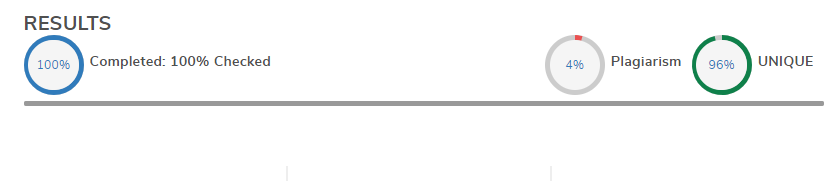
\includegraphics[width=4cm]{figures/Tugas1/1174062/plagiat.png}
	\centering
	\caption{Gambar Plagiat}
\end{figure}